\newpage
\section{Green Sustainability}
\label{sec:greensus}
The management of environmental aspects in a public transport company is aimed at their continuous improvement in terms of elimination, reduction or improvement of performance.

For uniform, transparent, goal-oriented and regulation-compliant management, we have to use of a set of procedures built from initial environmental analyses. The main environmental aspects that can be identified among all the material issues are:
\begin{itemize}
    \item Emissions into the atmosphere
    \item Energy Utilization
    \item Water Waste
    \item Waste Production
    \item Use of raw materials and natural resources
    \item Soil Contamination
    \item Dust, odors, vibrations, noise and visual impact problems
\end{itemize}

The significance of impacts can be assessed according to typical environmental analysis criteria, related to the severity, size and frequency of events, taking into account their controllability, applicable legal requirements and the expectations of stakeholders - local communities, employees and public administration. 
The Sustainable Development Goals \ref{ch:Innovative} considered under this aspect are mainly five:
\begin{itemize}
    \item \textbf{n°6 – Clean Water and Sanitation}, for what concerns water waste and overall consumption
    \item \textbf{n°7 – Affordable and Clean Energy}, in particular, considering all the types of energy consumption that a public transport service company have
     \item \textbf{n°11 – Sustainable Cities and Communities}, in particular the 11.6, concerning the emission environmental impact on cities
    \item \textbf{n°12 – Responsible Consumption and Production}, for what concerns raw materials consumption and waste management
    \item \textbf{n°13 – Climate Action}, to combat climate change taking into account all the aspects related to rolling stock, atmospheric and greenhouse emissions
\end{itemize}

\begin{figure}[!ht]
    \centering
    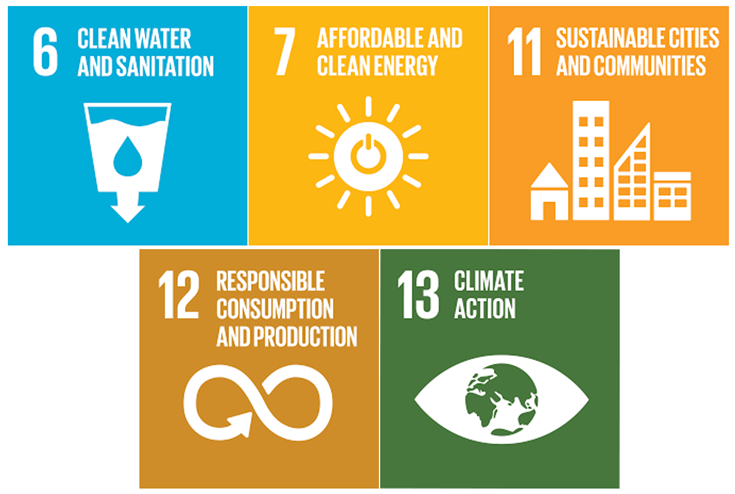
\includegraphics[width=1\textwidth]{Images/Green Sustainability/SDGs green.png}
    \caption{Green Sustainability SDGs}
    \label{fig:grsussdg}
\end{figure}

Regarding the five areas of interest in the SDGs \ref{fig:grsussdg}, it can be built a set of KPIs according to the goals previously stated.
We have decided to analyze three big groups of aspects related to the green sustainability:

\begin{itemize}
    \item \textbf{Energy Consumption} will focus on the amount of energy consumed and how it is distributed among all the activities that a PTO has to undertake. The aim is to reduce the consumption in the most efficient way.
    \item \textbf{Emissions} is one of the major topics related to Green Mobility and it is clearly essential to assess its problem and some way to keep track of it.
    \item \textbf{Waste} will be the last aspects taken into account, where we will focus on how to optimize both residual waste and water discharges.
\end{itemize}

\subsection{Energy Consumption}
\label{subsec:enecons}
Referring at the SDG number 7 \ref{par:onuobjectives}, by 2030 companies have to significantly increase the share of renewable in the global energy mix and double the global rate of energy efficiency improvement.
Energy consumption is mostly derived from bus fuels, which can be reduced through fleet renewal, maintenance activities and improved driving style. In addition to the consumption of buses, other sources of consumption have to be monitored, such as the electricity, natural gas and heating oil at the operational sites.
Looking at the overall activities that a company can perform, here in the table \ref{tab:sourceconsumption} are listed some of the main sources of consumption:

\begin{table}[!ht]
\centering
\begin{tabular}{l|l|}
\cline{2-2}
                                            & \cellcolor{bluepoli!40}Consumption   of:                                                                                 \\ \hline
\multicolumn{1}{|l|}{Running Buses}         & \begin{tabular}[c]{@{}l@{}}Fuel (diesel and natural gas)\\ Urea (Ad Blue)\\ Antifreeze\\ Lubricants\\ Tyres\end{tabular} \\ \hline
\multicolumn{1}{|l|}{Bus Maintenance}       & \begin{tabular}[c]{@{}l@{}}Spare parts\\ Electrical energy\end{tabular}                                                  \\ \hline
\multicolumn{1}{|l|}{Vehicle Cleaning}      & \begin{tabular}[c]{@{}l@{}}Water resources\\ Electrical energy\\ Detergent consumption\end{tabular}                      \\ \hline
\multicolumn{1}{|l|}{Refuelling}            & Electrical energy                                                                                                        \\ \hline
\multicolumn{1}{|l|}{Vehicle Storage}       & \begin{tabular}[c]{@{}l@{}}Soil\\ Electrical energy\end{tabular}                                                         \\ \hline
\multicolumn{1}{|l|}{Administration}        & \begin{tabular}[c]{@{}l@{}}Methane\\ Soil   \\ Electrical energy\\ Office supplies\end{tabular}                          \\ \hline
\multicolumn{1}{|l|}{\begin{tabular}[c]{@{}l@{}}Supply of goods, \\ materials and services\end{tabular}} & Fuel, Electrical energy, Office supplies                                                               \\ \hline
\end{tabular}
\caption{Main Sources of Consumption for a LPT company}
\label{tab:sourceconsumption}
\end{table}

With that in mind we can identify a set of indicators that can help monitor all of those aspects:
\begin{itemize}
    \item Gasoline and Methane consumption in GJ per km traveled by year
    \item Electrical Energy share usage with respect to previous years
    \item Green Energy used in each activity share
    \item Electricity Consumption share for electricity and heating of offices and sites compared to total energy consumption
    \item Green or Renewable fuel share over the totality of fuel used
    \item Energy Consumption share in relation to every km traveled with respect to the previous year
\end{itemize}

\subsection{Atmosphere and GHG Emissions}
\label{subsec:ghgemissions}
Between 1990 and 2018, emissions of all greenhouse gases in Italy decreased from 516 to 428 million tonnes of CO2 equivalent, a change achieved mainly by reducing carbon dioxide emissions, which contribute 81.4 \% of the total. Emissions in 2015 were 17.1\% lower than in 1990.

\begin{figure}[!ht]
    \centering
    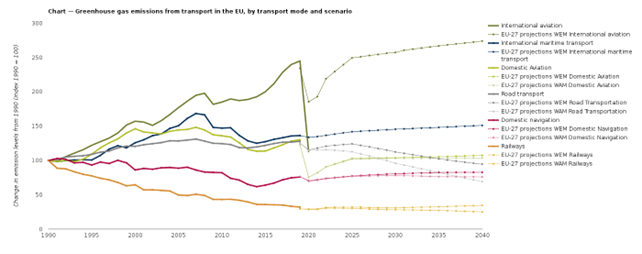
\includegraphics[width=1\textwidth]{Images/Green Sustainability/GHG emission.png}
    \caption{Greenhouse gas emissions from transport in the EU, by transport mode and scenario \cite{GreenhouseScenario}}
    \label{fig:ghgemissions}
\end{figure}

The energy production and transport sectors are the most important, contributing half of the national climate gas emissions. Compared to 1990, however, GHG emissions from the transport sector show a slight increase (3.2\%), while emissions from energy production and industrial installations are clearly decreasing (-23.7\% and -38.9\% respectively).

In this scenario, sustainable mobility is destined to play an important role since the increase in Local Public Transport can make a significant contribution to reducing emissions: Arriva therefore has to contribute to the transition to more energy and emission-efficient transport.
There are some actions that the company can undertake in order to commit gradually to this cause, such as:
\begin{itemize}
    \item Identify the activities that produce direct and indirect emissions both at atmospheric level and at greenhouse level
    \item Monitor and analysis of the emissions produced
    \item Implement projects and actions aimed at reducing them as well as measuring their effectiveness
    \item Raise internal and external awareness of this issue through reporting and communication to the stakeholders.
\end{itemize}

Greenhouse gas emissions can be reported in accordance with the GHG protocol (Greenhouse Gas protocol) \cite{ghgprotocol} which provides for the distinction into three categories:
\begin{description}
   \item[Scope 1] Direct emissions from the combustion of fossil fuels (diesel and natural gas) for road transport - bus fleet and car fleet - for the production of thermal energy and emissions of refrigerant gases from air conditioning systems. 
   \item[Scope 2] Emissions resulting from the production of electricity taken from the grid and consumed for the operation of plants and for lighting; the company is indirectly responsible for the emissions generated by the energy supplier for the production of the energy required. 
   \item[Scope 3] Indirect emissions, other than those from electricity consumption, which are a consequence of the company's activities and which arise from sources not owned or controlled by other organizations. The boundary of Scope 3 is defined by the organization and generally includes what can be quantified and influenced by the company.
\end{description}

As a partial solution for direct atmosphere emissions from the rolling stock, vehicles can be equipped with the innovative SCR - Selective Catalytic Reduction - system, which uses urea-based liquid, to reduce exhaust emissions in terms of particulate matter and nitrogen oxides. The system is able to reduce harmful substances in the exhaust gas of diesel vehicles by up to 80 per cent.

Wanting to quantify all of that, here below are listed some example KPIs:
\begin{itemize}
    \item Emissions of greenhouse gases (CO2, CFCs, CH4, etc.) per passenger transported or per km travelled
    \item Generic emissions (PM, VOCs, NOx, CO, etc.) per passenger transported or per km travelled
    \item Air quality standards and management plans. 
    \item Rolling Stock share with Euro5, Euro6 or EEV motorization
    \item Total km travelled by low-impact buses share
\end{itemize}

\subsection{Water Discharges and Waste Management}
\label{subsec:water}
The production of waste mainly originates from maintenance activities and bus washing. Improve the quality of water discharges from washing vehicles that may contain pollutants, such as hydrocarbons, oils and various powders is a main component of the green approach of a company Along with adequate purification plants regular inspections of the plants should be carried out, directly by the company. In the event of an emergency situation, all activities that produce water to be purified destined for the plant concerned should be suspended until the plant is operational again.

Purifiers and absorbent material will produce sludge, extracted during inspections and maintenance, which have to be stored in the plants themselves or in labeled containers at each site. The frequency of interventions has to be established on the basis of the indications in the maintenance booklets and those provided by the installer, as well as the actual use of the systems.

Storm water runoff from forecourt areas should be conveyed to plants for treatment, as required by regulations. To avoid possible contamination of runoff water the PTO can take some precautionary measures, such as:
\begin{itemize}
    \item Workshop activities have to take place in covered areas without sumps
    \item Waste storage have to takes place in covered areas and containers
    \item Storage areas that could give rise to environmental impacts on water discharges must be included in a water discharge monitoring plan
    \item Sumps and collection tanks must be inspected periodically and cleaned at least once a year
 \end{itemize}

According to all the procedures listed above, we have selected a list of KPIs that could be useful to track down this particular topic inside the company:

\begin{itemize}
    \item Liters shares of reused water
    \item Liters of storm water saved per year
    \item Tons of waste generated per year
    \item Mean time to inspection on service hours
    \item Percentage of hazardous waste recovered
    \item Tons of waste produced per 1000km traveled
\end{itemize}

\subsection{Mock Up Dashboard}
As per the previous chapter \ref{sec:newtech}, the aim of this is to built and visualize some mock-up dashboard pages, starting from the KPIs listed above in the previous paragraphs.

Also for this section, all pages are a mock-up also for what concerns the data present in he graphs, which may appear not close to the reality and made on purpose to talk about their benefits.

\newpage

\newpage
\begin{landscape}
\thispagestyle{empty}
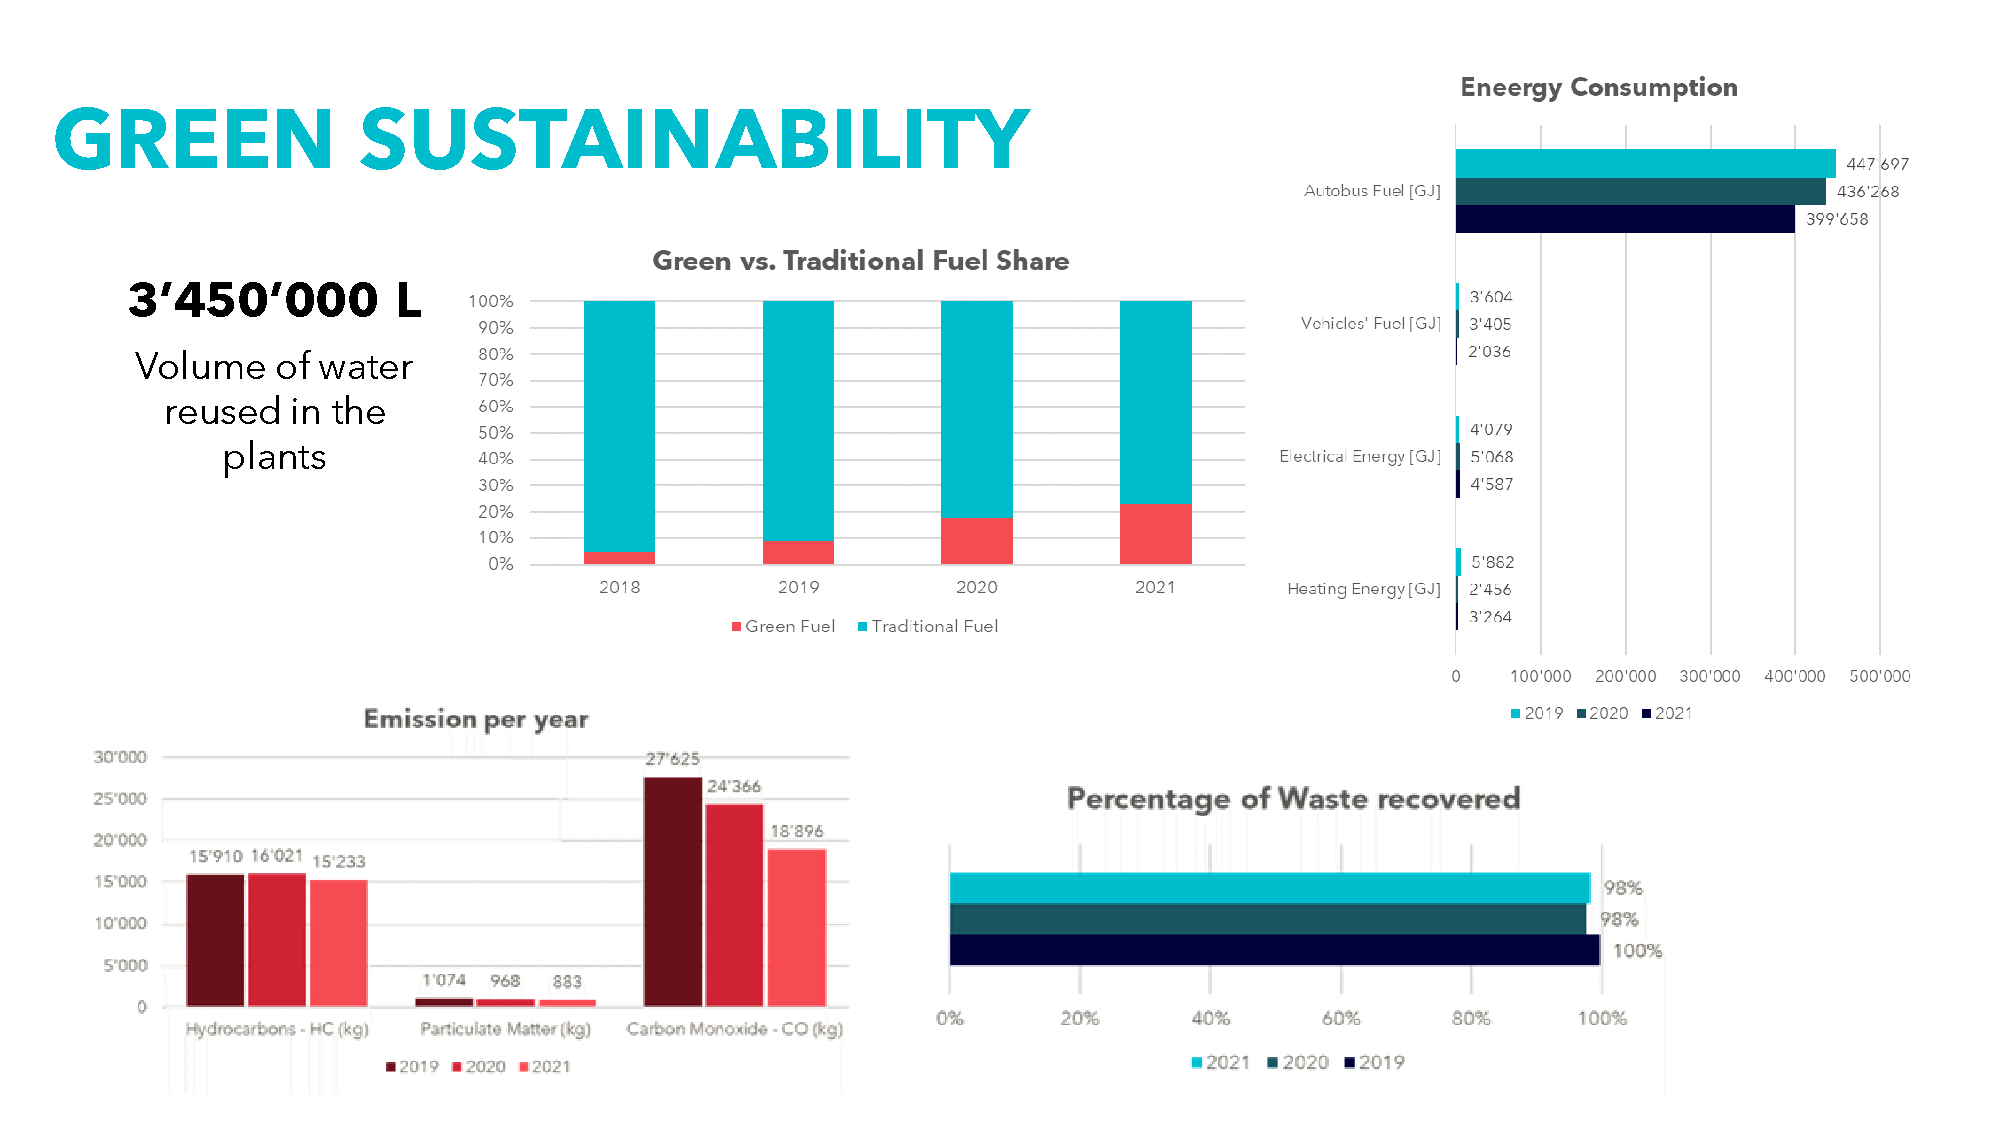
\includepdf[angle=90, pagecommand={\null\enlargethispage{3\baselineskip}\vfill\captionof{figure}{Green Sustainability page}\label{fig:work}}]{mockup/green.pdf}
\end{landscape}

\subsubsection{Green Sustainability}
This page mainly helps the observer to look at the development of green indicators by comparing values from year to year. A much more specific set-up could also be devised, to, for example, follow the trend of emissions, energy consumed, etc., on a daily or weekly basis during the year; in this case it would also be possible to activate preventive measures in case the values are too high compared to average trends or new limits imposed by regulation.
Having a clear view of how emissions and the quantity of environmentally friendly vehicles are being managed guarantees a strategic advantage at the planning level.

In addition, data on emissions or consumption can also be useful with a much higher frequency of collection, so as to be prepared in case the PTA requires immediate changes, such as a restriction on the circulation of certain types of vehicles for a few days to reduce smog in residential areas.
 
